% Chapter 12

\chapter{Análisis y Resultados} % Chapter title

\label{ch:analisis_resutados} % For referencing the chapter elsewhere, use \autoref{ch:name} 

%----------------------------------------------------------------------------------------
\section{Prototipo CWC}
El prototipo de CWC se programó utilizando el lenguaje de programación Python. Además se utilizó una biblioteca llamada btpeer. Ésta biblioteca implementa un protocolo P2P, el cual permite el intercambio de archivos. En la figura \ref{cwc} se pude ver la interfaz prototipo para un cliente-servidor.

\begin{figure}[h]
  \centering
    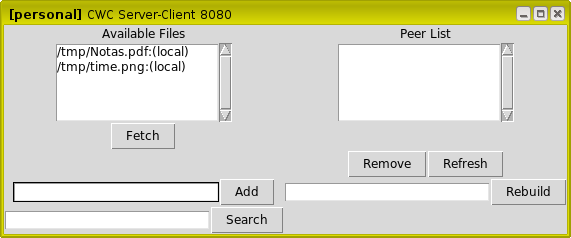
\includegraphics[scale=0.75]{gfx/cwc}
  \caption{Prototipo de CWC}
  \label{cwc}
\end{figure}

\section{Resultados de Rendimiento}

\begin{table}[h] %here h, t top, b bottom, p dedicated page on floats
\myfloatalign
\begin{tabular}{lcccc} \toprule % four columns, fist left, other ones centered. 
\tableheadline{Tipo de Archivo} & \tableheadline{Tamaño (MB)} & \tableheadline{Servidor Web} \\ \midrule
Imágenes & 2.4 & 12.6 s \\ 
Videos & 345.9 & 1802.1 s  \\
Documentos & 1.3 & 6.6s  \\
Instaladores & 34.6 & 181.2s  \\
\end{tabular}
\caption{Resultados del escenario Sin Web Caché}  
\label{tab:resultado_web}
\end{table}

\begin{table}[h] %here h, t top, b bottom, p dedicated page on floats
\myfloatalign
\begin{tabular}{lcccc} \toprule % four columns, fist left, other ones centered. 
\tableheadline{Tipo de Archivo} & \tableheadline{Tamaño (MB)} & \tableheadline{1 Nodo} & \tableheadline{2 nodos} & \tableheadline{3 nodos}\\ \midrule
Imágenes & 2.4  & 13.4 s & 12.9 s & 13.1 s \\ 
Videos & 345.9 & 1786.5 s &  902.8 s & 603.7 s \\
Documentos & 1.3 & 7.1 s & 6.9 s & 7.0 s \\
Instaladores & 34.6 & 168.4 s & 88.57 s & 58.2 s \\
\end{tabular}
\caption{Resultados del escenario Prototipo CWC}  
\label{tab:resultado_cwc}
\end{table}

\section{Análisis de rendimiento de velocidad del entorno de CWC}

Las herramientas seleccionadas para la medición del rendimiento fueron:
\begin{itemize}
\item Httperf: Se utilizó para medir el rendimiento del escenario Sin Web Caché
\item time: Se utilizó para medir el rendimiento del escenario del prototipo de CWC
\end{itemize}

Basado en la tabla \ref{tab:resultado_web} en combinación con la tabla \ref{tab:resultado_cwc} es posible concluir que conforme más grande sea el archivo la red P2P se comporta de una mejor manera. Por el contrario, esto no sucede con los archivos pequeños, pues estos archivos son servidos siempre desde un único nodo, según el protocolo. Por otro lado se sirvieron archivos pequeños desde distintas ubicaciones, y ésto no significó mayor mejora, en cuanto al tiempo de respuesta. 

\section{Resultados de Costo}

\begin{table}[h] %here h, t top, b bottom, p dedicated page on floats
\myfloatalign
\begin{tabular}{lcccc} \toprule % four columns, fist left, other ones centered. 
\tableheadline{Componente} & \tableheadline{Servidor Web} & \tableheadline{1 Nodo} & \tableheadline{2 nodos} & \tableheadline{3 nodos}\\ \midrule
Memoria & \$40  & \$40  & \$0 & \$0 \\ 
Procesador & \$120 & \$120 & \$0 & \$0 \\
Almacenamiento & \$55 & \$55 & \$0 & \$0 \\
Interfaz de Red & \$10 & \$40 & \$0 & \$0 \\
Total & \$255 & \$255 & \$0 & \$0 \\
\end{tabular}
\caption{Comparación de costos}  
\label{tab:resultado_costo}
\end{table}

%----------------------------------------------------------------------------------------

\section{Análisis de costos del Entorno de CW}

En el caso del CWC, basado en la tabla \ref{tab:resultado_costo}, es posible determinar que entre más nodos más barato es el mantenimiento del sitio. Esto pues, los nodos adicionales se componen de recursos que son cedidos a través de la comunidad. Por otro lado, también se puede concluir basado en la tabla \ref{tab:resultado_cwc} y la tabla \ref{tab:resultado_costo} que el costo decrece, y el servicio aumenta, si aumentamos el número de nodos conectados a la comunidad. 